%%%%%%%%%%%%%%%%%%%%%%%%%%%%%%%%%%%%%%
%%%%%%%%%%%%%%%%%%%%%%%%%%%%%%%%%%%%%%
% Do not edit the TeX file your work
% will be overwritten.  Edit the RnW
% file instead.
%%%%%%%%%%%%%%%%%%%%%%%%%%%%%%%%%%%%%%
%%%%%%%%%%%%%%%%%%%%%%%%%%%%%%%%%%%%%%






\begin{knitrout}
\definecolor{shadecolor}{rgb}{0.969, 0.969, 0.969}\color{fgcolor}\begin{figure}[!h]

{\centering 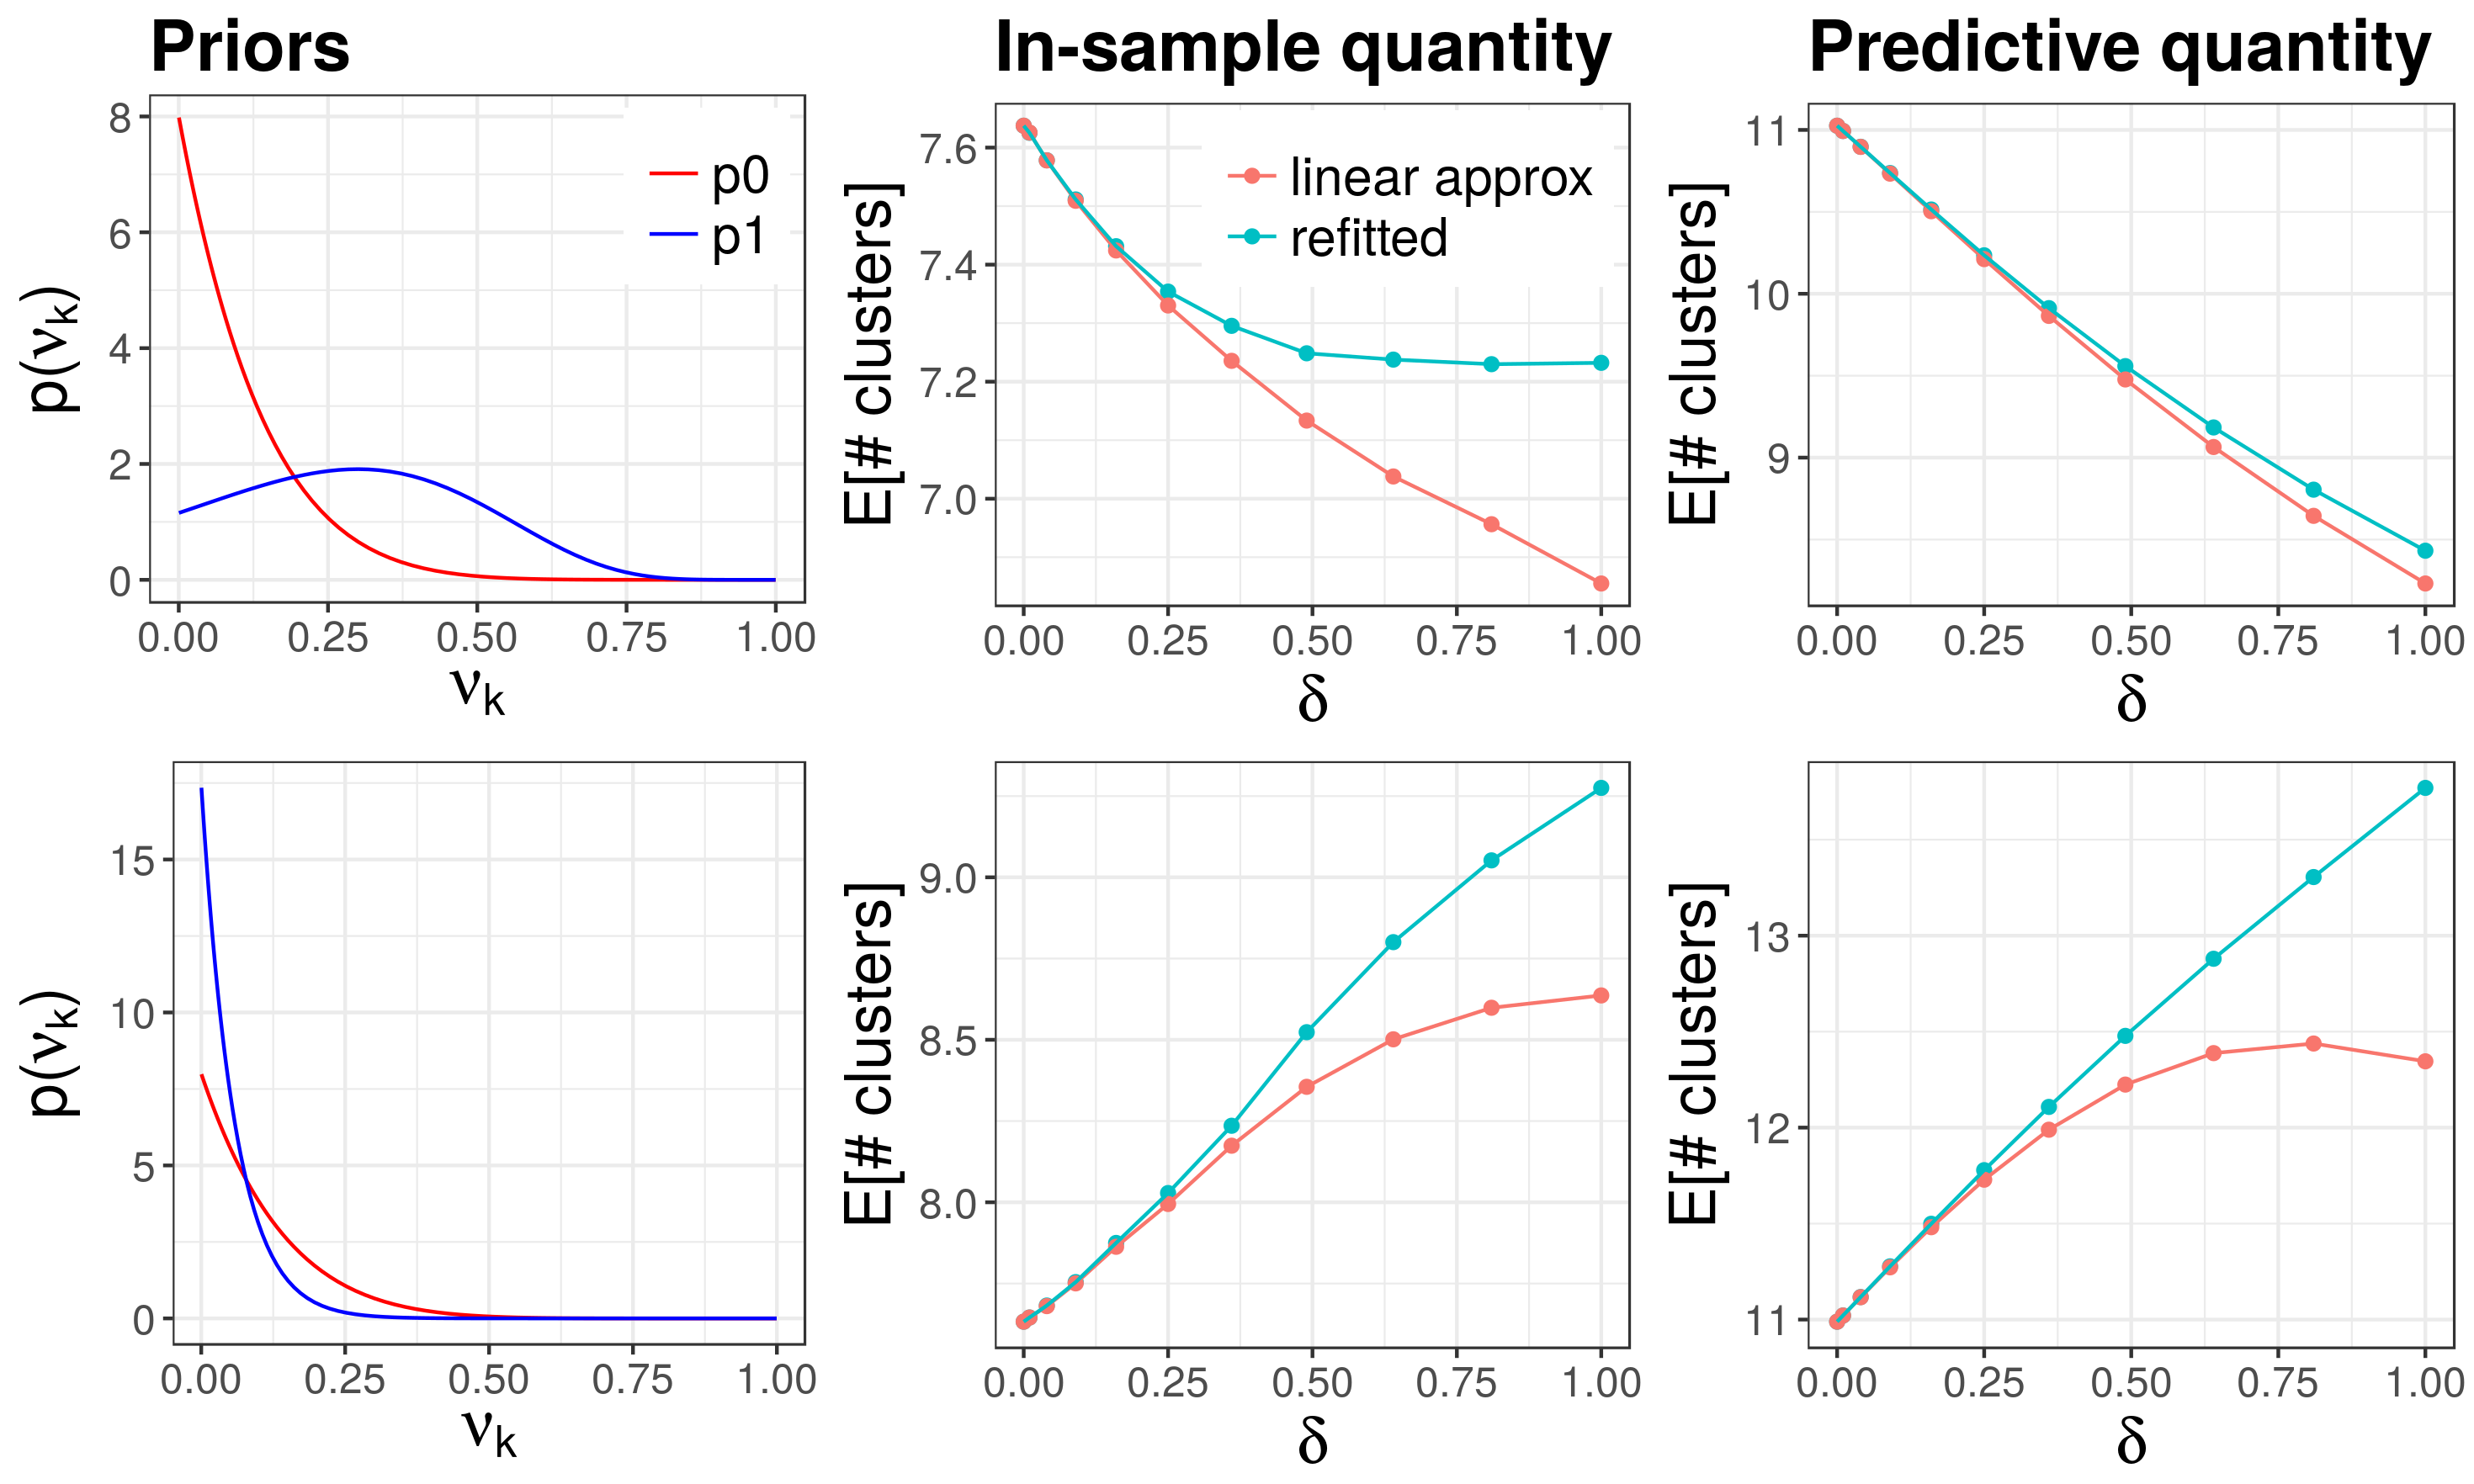
\includegraphics[width=0.98\linewidth,height=0.588\linewidth]{figure/functional_sens_plot_thresh0-1} 

}

\caption{\label{fig:func_sens_e_num_clusters_thresh0}
Left column: the original prior $p_{0k}$ in orange,
the perturbed prior $p^c_k$ in green. Right: linearly approximated vs.
re-fitted expected number of clusters after the pertubation.  }\label{fig:functional_sens_plot_thresh0}
\end{figure}


\end{knitrout}
%



\begin{knitrout}
\definecolor{shadecolor}{rgb}{0.969, 0.969, 0.969}\color{fgcolor}\begin{figure}[!h]

{\centering \includegraphics[width=0.98\linewidth,height=0.588\linewidth]{figure/functional_sens_plot_thresh3-1} 

}

\caption{\label{fig:func_sens_e_num_clusters_thresh3}
Left column: the original prior $p_{0k}$ in orange,
the perturbed prior $p^c_k$ in green. Right: linearly approximated vs.
re-fitted expected number of clusters after the pertubation.  }\label{fig:functional_sens_plot_thresh3}
\end{figure}


\end{knitrout}
